\documentclass[slidestop,compress,xcolor=table,mathserif,hyperref={bookmarks=false}]{beamer}
\usetheme{TACC}

\usepackage{tikz}
\usetikzlibrary{automata,shapes,arrows}
\usepackage{lmodern}
\usepackage[overlay]{textpos}
\usepackage[applemac]{inputenc}
\usepackage{pgfpages}
\usepackage{multirow}

\newenvironment<>{varblock}[2][.9\textwidth]{
  \setlength{\textwidth}{#1}
  \begin{actionenv}#3
    \def\insertblocktitle{#2}
    \par
    \usebeamertemplate{block begin}}
  {\par
    \usebeamertemplate{block end}
  \end{actionenv}}

\author{\textbf{\Large Jim Browne, Ashay Rane and Leo Fialho}}
\begin{document}

\AtBeginSection[]{
	\frame<beamer>{
		\frametitle{Agenda}
		\begin{columns}[c]
			\begin{column}{0.5\textwidth}
				\tableofcontents[currentsection,subsectionstyle=shadow/hide/hide]
			\end{column}
			\begin{column}{0.5\textwidth}
				\pgfuseimage{configuration}
			\end{column}
		\end{columns}
	}
}

%------------------------------------------------------------
\pgfdeclareimage[interpolate=true,width=5cm]{logo_TACC}{figures/tacc}
\pgfdeclareimage[interpolate=true,width=5cm]{logo_UT}{figures/ut}
\pgfdeclareimage[interpolate=true,width=1.5cm]{logo_TACC_small}{figures/tacc}
\pgfdeclareimage[interpolate=true,width=1cm]{logo_UT_small}{figures/ut}
\pgfdeclareimage[interpolate=true,width=6cm]{configuration}{figures/configuration}

%------------------------------------------------------------
\title{\textbf{\LARGE Performance Optimization\\with PerfExpert and MACPO\\}}
\date{\textbf{\Huge ICS 2013} \\ \ \\ \ \\ \pgfuseimage{logo_TACC} \ \ \pgfuseimage{logo_UT}}
\logo{\pgfuseimage{logo_TACC_small} \ \ \ \pgfuseimage{logo_UT_small}}
\frame[plain]{\titlepage}

%------------------------------------------------------------
\section{Introduction}
\subsection{Agenda}

\frame{\frametitle{Agenda} \pause
	\begin{block}{In the morning:}
		\textbf{09:00} Introduction and motivation \textit{[Jim]} \\[2mm] 
		\textbf{09:20} What PerfExpert can provide to you? \textit{[Leo]} \\[2mm]
		\textbf{09:30} Demo \textit{[Leo]} \\[2mm]
		\textbf{09:45} How PerfExpert does that? (opening Pandora's box) \textit{[Leo]} \\[2mm]
		\textbf{10:15} Extending PerfExpert \textit{[Leo]} \\[2mm]
		\textbf{10:30} (Coffee?) break \textit{[everyone, including you]} \\[2mm]
		\textbf{10:45} Hands on tutorial \textit{[all the team]} \\[2mm]
		\textbf{11:45} Morning closure \textit{[all the team]} \\[2mm]
	\end{block}
}

\frame{\frametitle{Agenda} \pause
	\begin{block}{In the afternoon:}
		\textbf{01:30} What MACPO can provide to you? \textit{[Ashay]} \\[2mm]
		\textbf{02:00} Demo \textit{[Ashay, Jim]} \\[2mm]
		\textbf{02:30} How MACPO does that? \textit{[Ashay]} \\[2mm]
		\textbf{03:15} (Coffee?) break \textit{[everyone, including you]} \\[2mm]
		\textbf{03:30} Hands on tutorial \textit{[Ashay]} \\[2mm]
		\textbf{04:00} Selecting code segments to run on GPUs/accelerators \textit{[Jim]} \\[2mm]
		\textbf{04:30} Enhancing PerfExpert with MACPO analysis \textit{[all the team]} \\[2mm]
		\textbf{04:45} Afternoon closure and future work \textit{[all the team]} \\[2mm]
	\end{block}
}

\subsection{Overview}
\frame{\frametitle{Overview: why PerfExpert?} \pause
	\begin{block}{Problem: HPC systems operate far below peak} \pause
		\begin{itemize}
			\item Chip/node architectural complexity is growing rapidly \\[2mm] \pause
			\item Performance optimization for these chips requires deep knowledge of architectures, code patterns, compilers, etc. \\[2mm]
		\end{itemize}
	\end{block}

	\begin{exampleblock}{Performance optimization tools} \pause
		\begin{itemize}
			\item Powerful in the hands of experts \\[2mm] \pause
			\item Require detailed performance and system expertise \\[2mm] \pause
			\item HPC application developers are domain experts, not computer gurus \\[2mm] \pause
		\end{itemize}
	\end{exampleblock}

	\begin{alertblock}{Result: Many HPC programmers do not use these tools}
		\centering (seriously)
	\end{alertblock}
}

\frame{\frametitle{Goal for PerfExpert: democratize optimization!} \pause
	\begin{block}{Subgoals:} \pause
		\begin{itemize}
			\item Make use of the tool as simple as possible \\[2mm] \pause
			\item Start with only chip/node level optimization \\[2mm] \pause
			\item Make it adaptable across multiple architectures \\[2mm] \pause
			\item Design for extension to communication and I/O performance \\[2mm] \pause
		\end{itemize}
	\end{block}

	\begin{exampleblock}{How to accomplish?} \pause
		\begin{itemize}
			\item Formulate the performance optimization task as a workflow of subtasks \\[2mm] \pause
			\item Leverage the state-of-the-art: Build on the best available tools for the subtasks to minimize the effort and cost of development \\[2mm] \pause
			\item Automate the entire workflow \\[2mm] \pause
		\end{itemize}
	\end{exampleblock}
}

\subsection{Introduction}
\frame{\frametitle{Introduction}
	\begin{block}{The four stages of automatic performance optimization:} \pause
		\begin{itemize}
			\item Measurement and attribution (1) \\[2mm] \pause
			\item Analysis, diagnosis and identification of bottlenecks (2) \\[2mm] \pause
			\item Selection of effective optimizations (3) \\[2mm] \pause
			\item Implementation of optimizations (4) \\[2mm] \pause
		\end{itemize}
	\end{block}

	\begin{exampleblock}{Use of State-of-the-Art:} \pause
		\begin{itemize}
			\item HPCToolkit, \textbf{MACPO} based on ROSE (1) \\[2mm] \pause
			\item \textbf{PerfExpert Team} (2 and 3) \\[2mm] \pause
			\item \textbf{PerfExpert Team} based on ROSE, PIPS, Bison and Flex (4)\\[2mm] \pause
		\end{itemize}
	\end{exampleblock}
}

\frame{\frametitle{Introduction}
	\begin{block}{Uniqueness of PerfExpert:} \pause
		\begin{itemize}
			\item Nearly complete optimization first three stages of optimization for chip/node level \\[2mm] \pause
			\item Framework for implementing optimizations is complete and several optimizations are completed \\[2mm] \pause
			\item Integrates code segment focused and data structure based measurements (\textbf{MACPO})\\[2mm] \pause
			\item Workflow will apply to communication and I/O optimization as well \\[2mm] \pause
		\end{itemize}
	\end{block}
}

\frame{\frametitle{Introduction}
	\begin{block}{Unique properties of MACPO:} \pause
		\begin{itemize}
			\item Multicore resolved traces \\[2mm] \pause
			\item Code segment local measurement \\[2mm] \pause
			\item Data structure specific traces \\[2mm] \pause
			\item Order of magnitude lower overhead of measurement \\[2mm] \pause
			\item More accurate (associative) cache models \\[2mm] \pause
			\item Strides by data structure and code segment \\[2mm] \pause
			\item Architecture ``independent'' metrics \\[2mm] \pause
		\end{itemize}
	\end{block}
}

%------------------------------------------------------------
\section{PerfExpert}
\subsection{What PerfExpert can provide to you?}

\frame{\frametitle{What PerfExpert can provide to you?}
	\begin{block}{Performance report:} \pause
		\begin{itemize}
			\item Identification of bottlenecks by relevance \\[2mm] \pause
			\item Performance analysis based on performance metrics \\[2mm] \pause
			\item Recommendations for optimization \\[2mm] \pause
		\end{itemize}
	\end{block}

	\begin{exampleblock}{There are three possible outputs:} \pause
		\begin{itemize}
			\item Performance report only \\[2mm] \pause
			\item List of recommendations \\[2mm] \pause
			\item Fully automated code transformation \\[2mm] \pause
		\end{itemize}
	\end{exampleblock}
}

\frame{\frametitle{What PerfExpert can provide to you?}
	\begin{block}{Performance report:} \pause
\texttt{\tiny Loop in function compute() at mm.c:8 (99.8\% of the total runtime)\\
===============================================================================\\
ratio to total instrns \ \ \ \ \ \ \%  0.........25...........50.........75........100\\
\ \ \ - floating point \ \ \ \ \ : \ 100 ***********************************************\\
\ \ \ - data accesses \ \ \ \ \ \ : \ \ 25 ************\\
* GFLOPS (\% max) \ \ \ \ \ \ \ \ : \ \ 12 ******\\
\ \ \ - packed \ \ \ \ \ \ \ \ \ \ \ \ \ : \ \ \ 0 *\\
\ \ \ - scalar \ \ \ \ \ \ \ \ \ \ \ \ \ : \ \ 12 ******\\
-------------------------------------------------------------------------------\\
performance assessment \ \ \ \ LCPI good......okay......fair......poor......bad....\\
* overall \ \ \ \ \ \ \ \ \ \ \ \ \ \ \ : \ 3.0 >>>>>>>>>>>>>>>>>>>>>>>>>>>>>>>>>>>>>>>>>>>>>>+\\
upper bound estimates\\
* data accesses \ \ \ \ \ \ \ \ \ : \ 9.6 >>>>>>>>>>>>>>>>>>>>>>>>>>>>>>>>>>>>>>>>>>>>>>+\\
\ \ \ - L1d hits \ \ \ \ \ \ \ \ \ \ \ : \ 0.9 >>>>>>>>>>>>>>>>>\\
\ \ \ - L2d hits \ \ \ \ \ \ \ \ \ \ \ : \ 1.8 >>>>>>>>>>>>>>>>>>>>>>>>>>>>>>>>>>>>>\\
\ \ \ - L2d misses \ \ \ \ \ \ \ \ \ : \ 6.9 >>>>>>>>>>>>>>>>>>>>>>>>>>>>>>>>>>>>>>>>>>>>>>+\\
* instruction accesses \ \ : \ 0.1 >\\
\ \ \ - L1i hits \ \ \ \ \ \ \ \ \ \ \ : \ 0.0 >\\
\ \ \ - L2i hits \ \ \ \ \ \ \ \ \ \ \ : \ 0.0 >\\
\ \ \ - L2i misses \ \ \ \ \ \ \ \ \ : \ 0.1 >\\
* data TLB \ \ \ \ \ \ \ \ \ \ \ \ \ \ : \ \ 4.6 >>>>>>>>>>>>>>>>>>>>>>>>>>>>>>>>>>>>>>>>>>>>>>+\\
* instruction TLB \ \ \ \ \ \ \ : \ \ 0.0 >\\
* branch instructions \ \ \ : \ 0.1 >>\\
\ \ \ - correctly predicted : \ 0.1 >>\\
\ \ \ - mispredicted \ \ \ \ \ \ \ : \ 0.0 >\\
* floating-point instr \ \ : \ 5.1 >>>>>>>>>>>>>>>>>>>>>>>>>>>>>>>>>>>>>>>>>>>>>>+\\
\ \ \ - fast FP instr \ \ \ \ \ \ : \ 5.1 >>>>>>>>>>>>>>>>>>>>>>>>>>>>>>>>>>>>>>>>>>>>>>+\\
\ \ \ - slow FP instr \ \ \ \ \ \ : \ 0.0 >\\
}
   \end{block}
}

\frame{\frametitle{What PerfExpert can provide to you?}
	\begin{block}{List of Recommendations:} \pause
\texttt{\tiny \#--------------------------------------------------\\
\# Recommendations for mm.c:8\\
\#--------------------------------------------------\\
\#\\
\# This is a possible recommendation for this code segment\\
\#\\
Recommendation ID: 31\\
Recommendation Description: change the order of loops\\
Recommendation Reason: this optimization may improve the memory access pattern and make it more cache and TLB friendly\\
Pattern Recognizers: c\_loop2 f\_loop2 \\
Code example:\\
loop i \{\\
\ \ loop j \{...\}\\
\}\\
 =====>
loop j \{\\
\ \ loop i \{...\}\\
\}\\
}
   \end{block}
}

\subsection{Demo: PerfExpert}

\frame{\frametitle{Short Demo}
	\vspace{2.5cm}
	\begin{center}
		\textit{\textbf{\Huge{Short demo}}}
	\end{center}
}

\subsection{How PerfExpert does that?}

\frame{\frametitle{How PerfExpert does that: The Big Picture}
	\begin{picture}(0,0)(0,0)
		\put(-28,-160){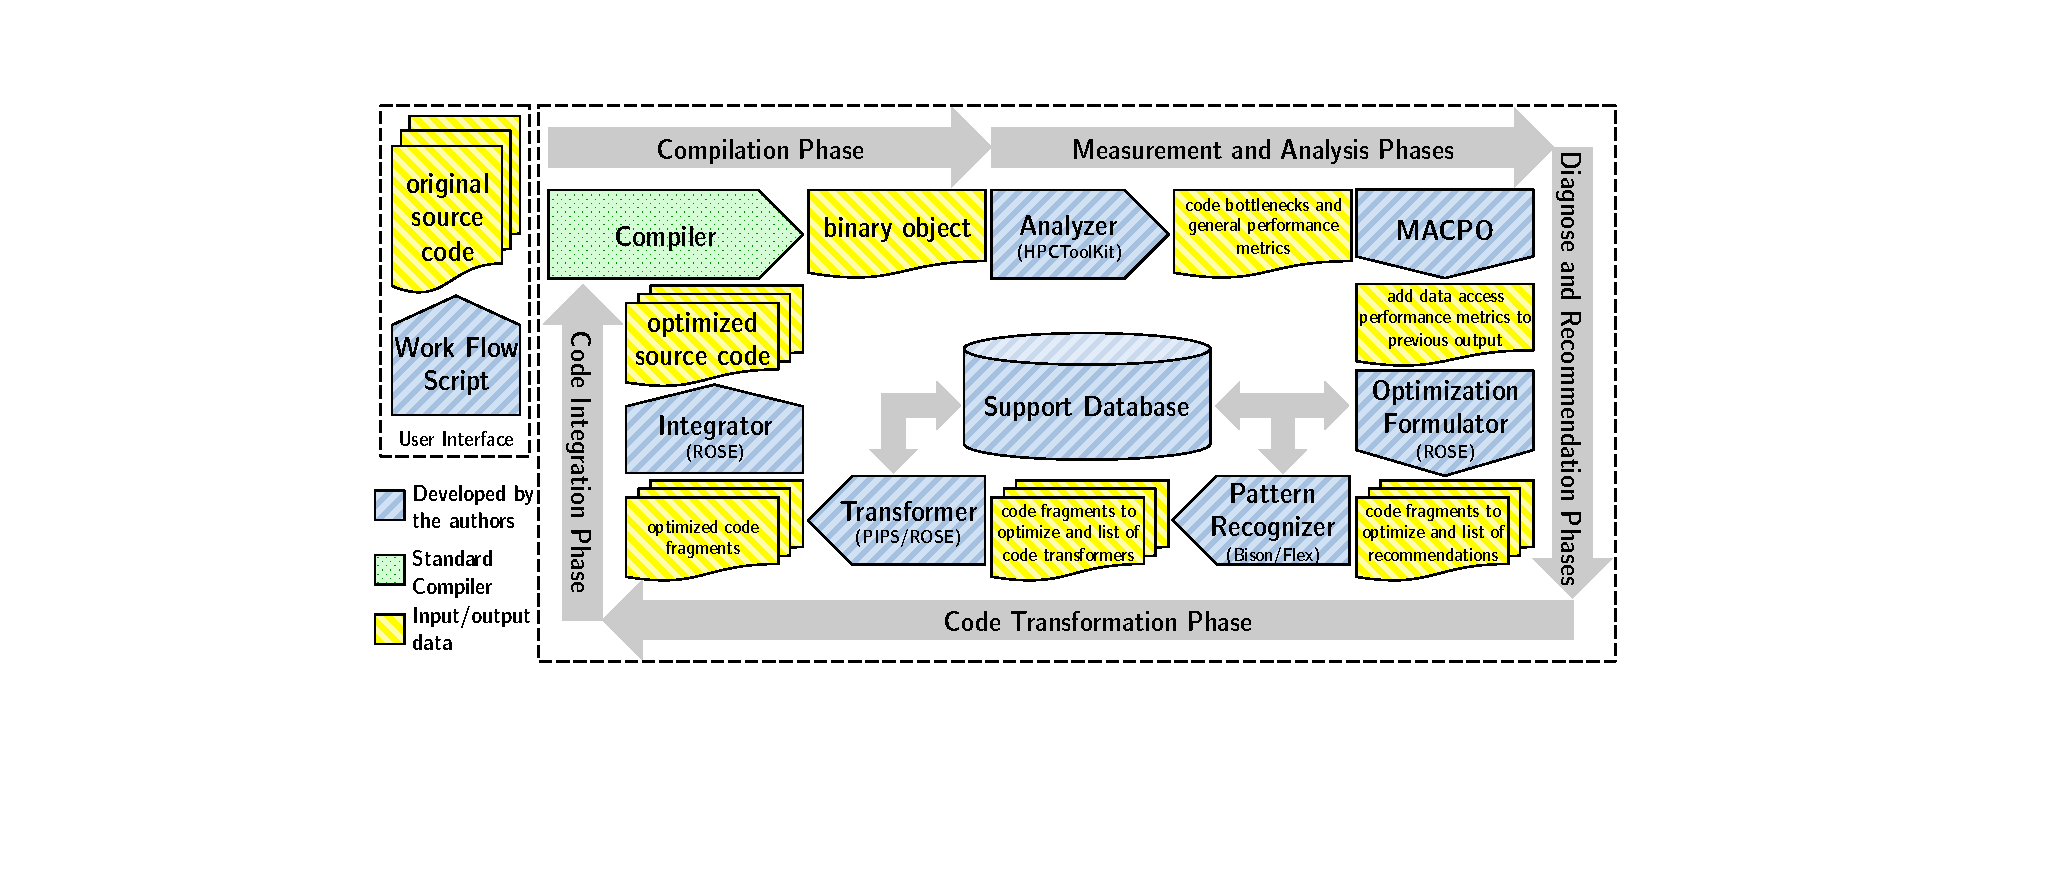
\includegraphics[width=12.8cm]{figures/pe_after}}
	\end{picture}
}

\frame{\frametitle{How PerfExpert does that: Work Flow Script}
	\begin{picture}(0,0)(0,0)
		\put(-28,-160){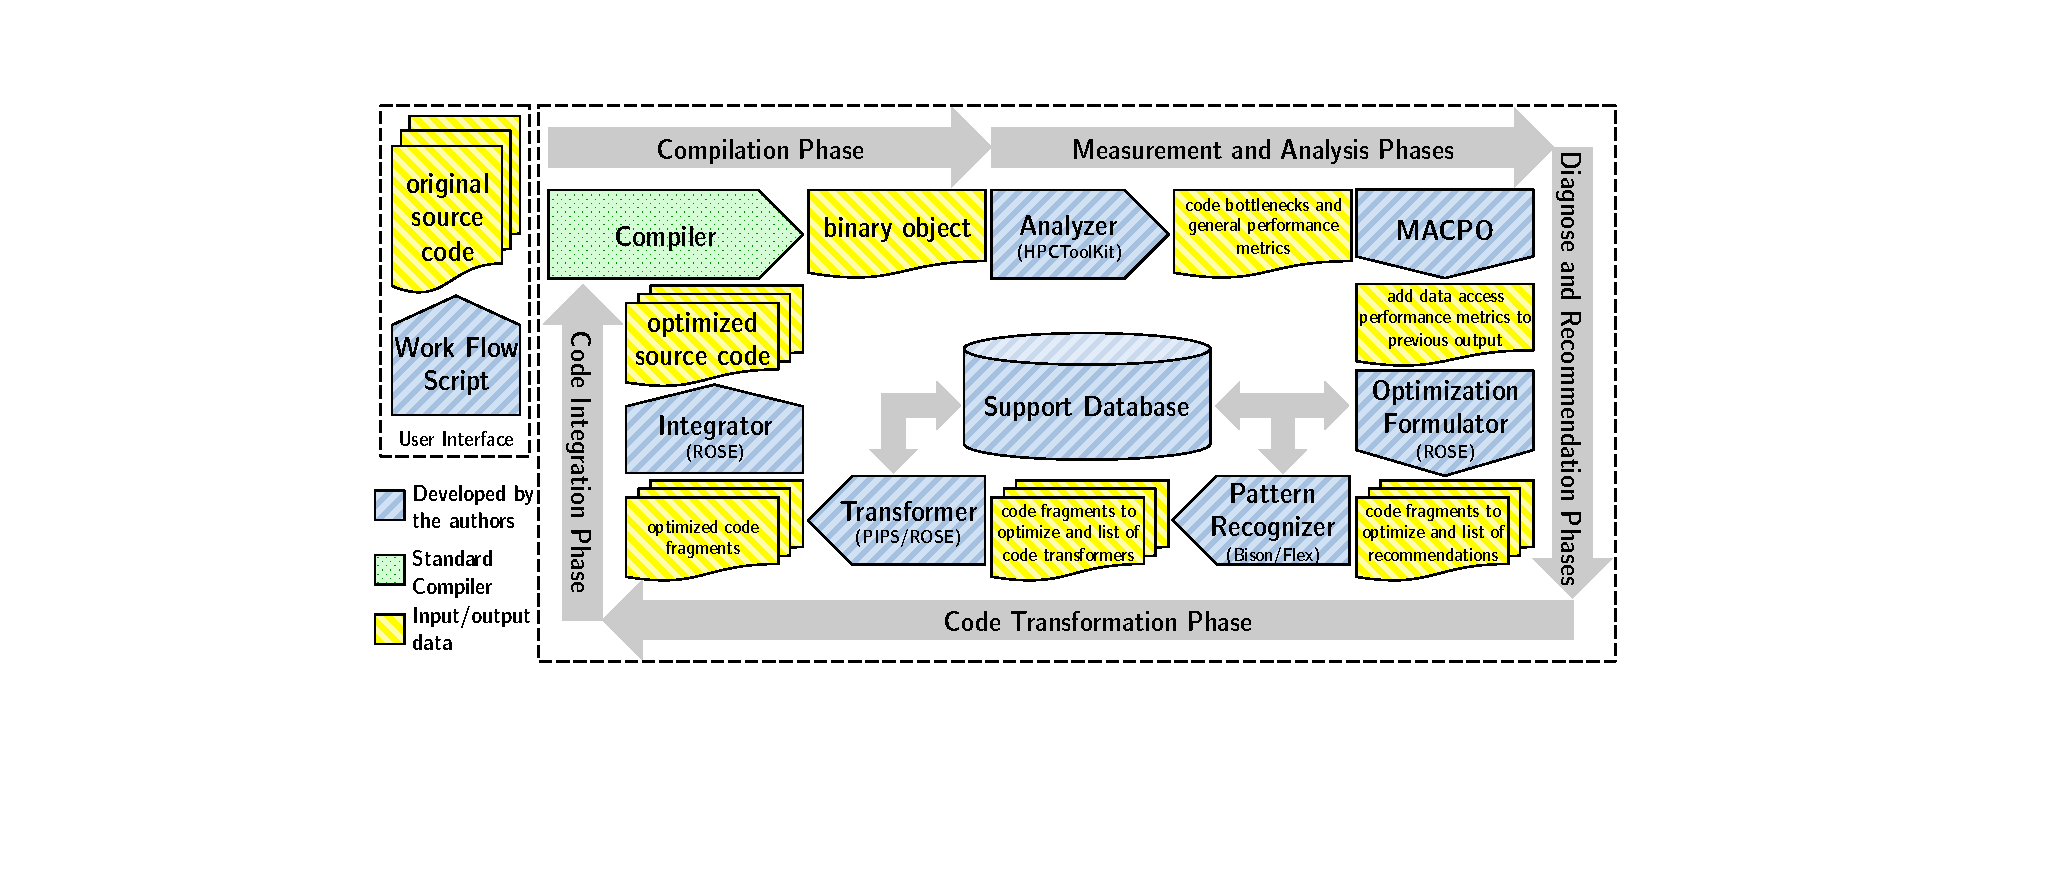
\includegraphics[width=12.8cm]{figures/pe_after}}
	\end{picture} \pause
	\begin{columns}[c]
		\begin{column}{0.09\textwidth}
		\end{column}
		\begin{column}{0.43\textwidth}
			\vspace{1.5cm}
			\begin{block}{}
				\begin{itemize}
					\item This is a shell script \\[2mm] \pause
					\item Accepts parameters \\[2mm] \pause
					\item Invokes all tools (including the compiler) \\[2mm] \pause
					\item Backward compatible \\[2mm]
				\end{itemize}
			\end{block}
		\end{column}
		\begin{column}{0.48\textwidth}
		\end{column}
	\end{columns}
}

\frame{\frametitle{How PerfExpert does that: Analyzer}
	\begin{picture}(0,0)(0,0)
		\put(-28,-160){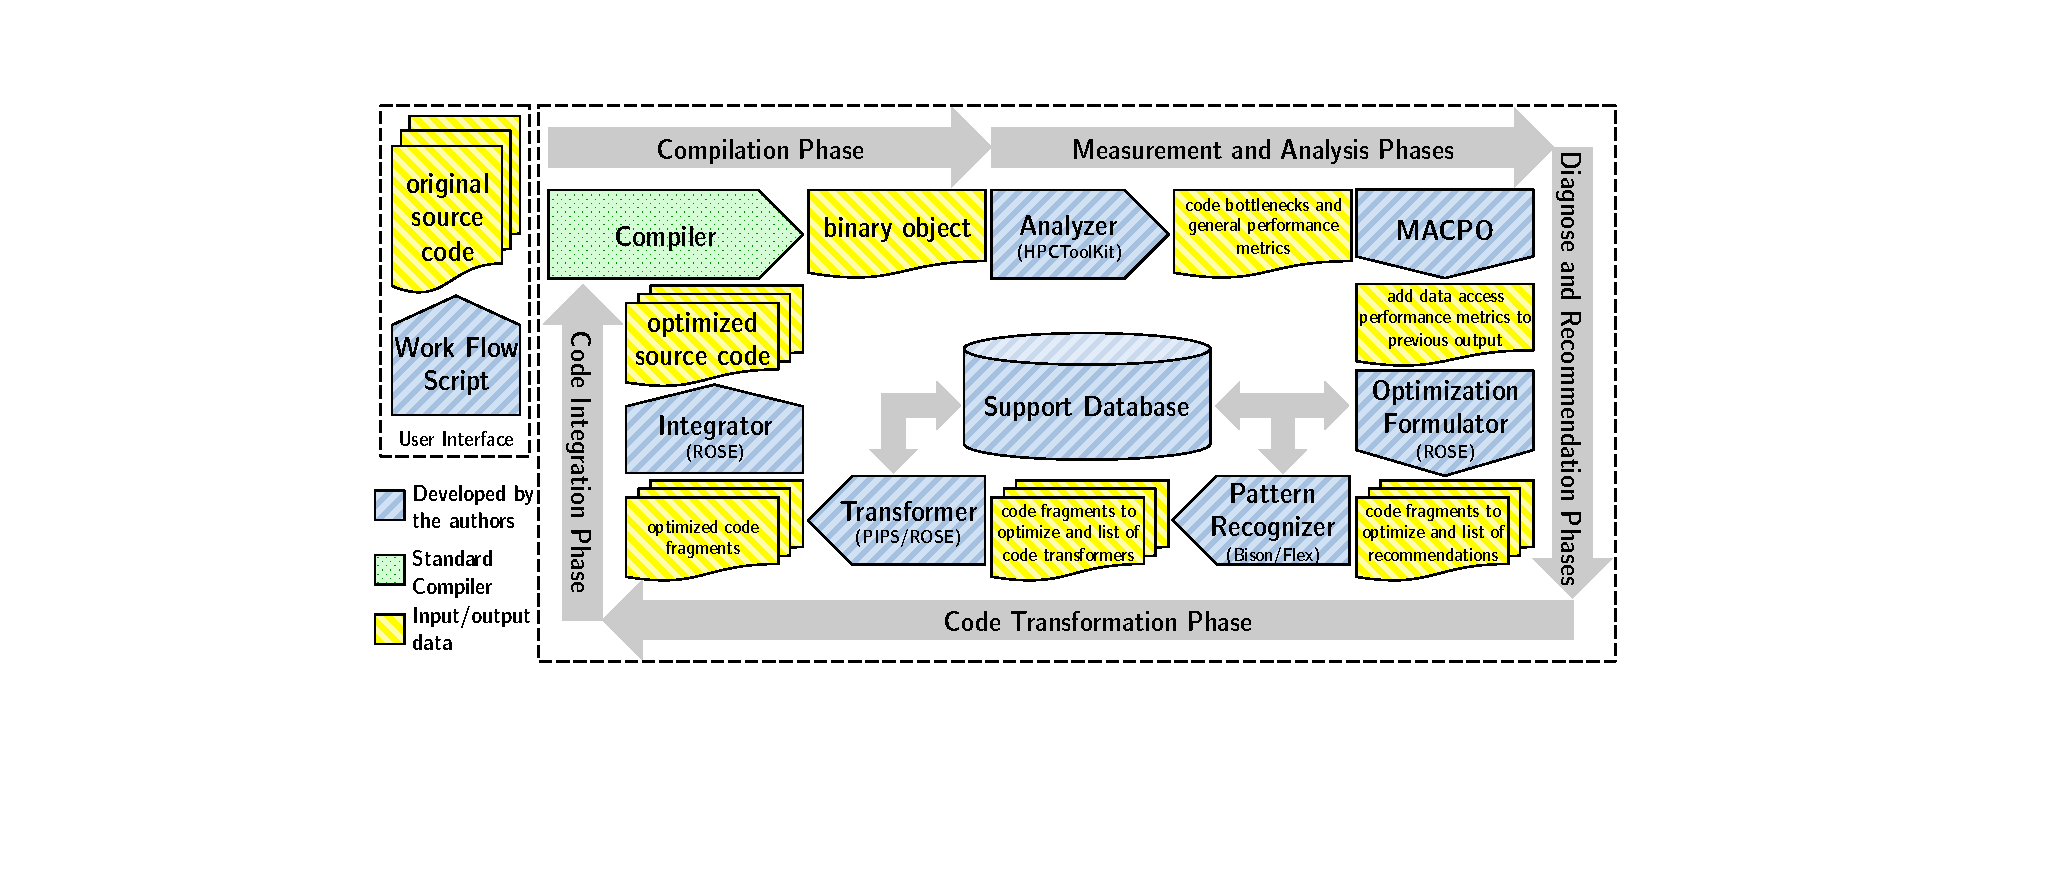
\includegraphics[width=12.8cm]{figures/pe_after}}
	\end{picture} \pause
	\begin{columns}[c]
		\begin{column}{0.35\textwidth}
		\end{column}
		\begin{column}{0.46\textwidth}
			\vspace{1.5cm}
			\begin{block}{}
				\begin{itemize}
					\item This is the old PerfExpert, minus ``recommender'' \\[2mm] \pause
					\item Based on HPCToolKit \\[2mm]
				\end{itemize}
			\end{block}
		\end{column}
		\begin{column}{0.19\textwidth}
		\end{column}
	\end{columns}
}

\frame{\frametitle{How PerfExpert does that: MACPO}
	\begin{picture}(0,0)(0,0)
		\put(-28,-160){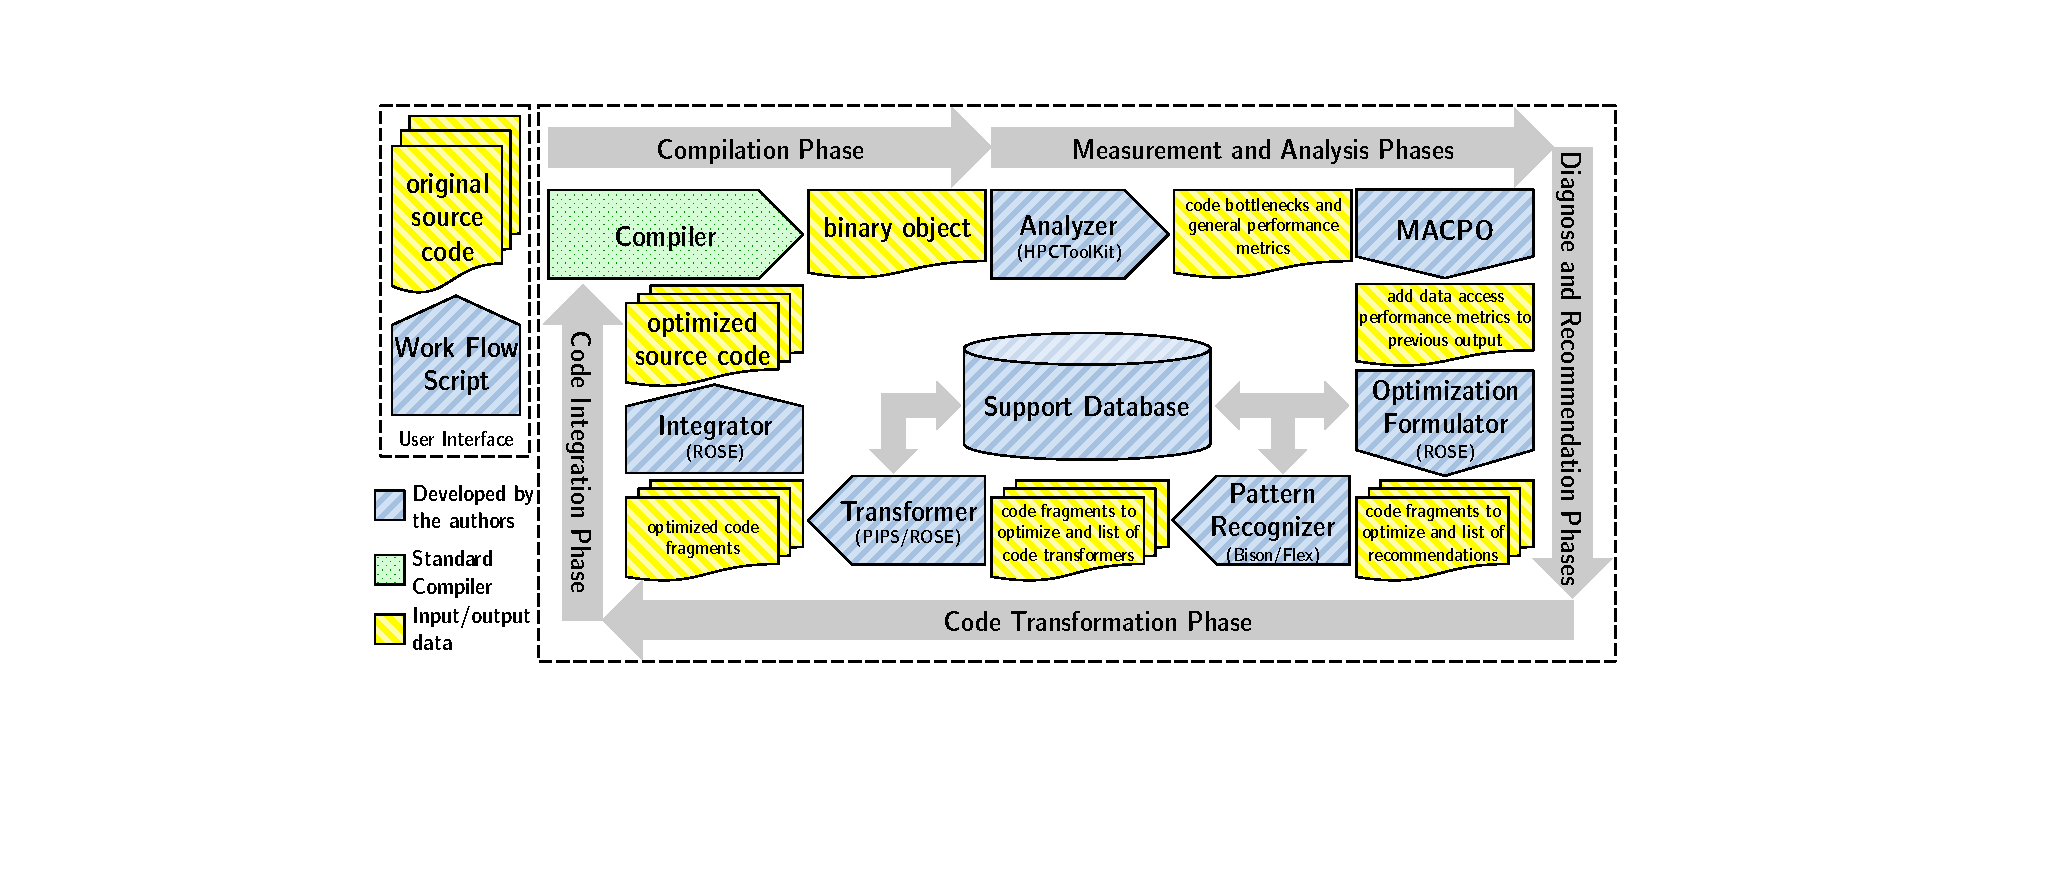
\includegraphics[width=12.8cm]{figures/pe_after}}
	\end{picture} \pause
	\begin{columns}[c]
		\begin{column}{0.35\textwidth}
		\end{column}
		\begin{column}{0.46\textwidth}
			\vspace{1.5cm}
			\begin{block}{}
				\begin{itemize}
					\item Enhances the set of metrics with data access performance metrics \\[2mm] \pause
					\item Based on ROSE \\[2mm]
				\end{itemize}
			\end{block}
		\end{column}
		\begin{column}{0.19\textwidth}
		\end{column}
	\end{columns}
}

\frame{\frametitle{How PerfExpert does that: Optimization Formulator}
	\begin{picture}(0,0)(0,0)
		\put(-28,-160){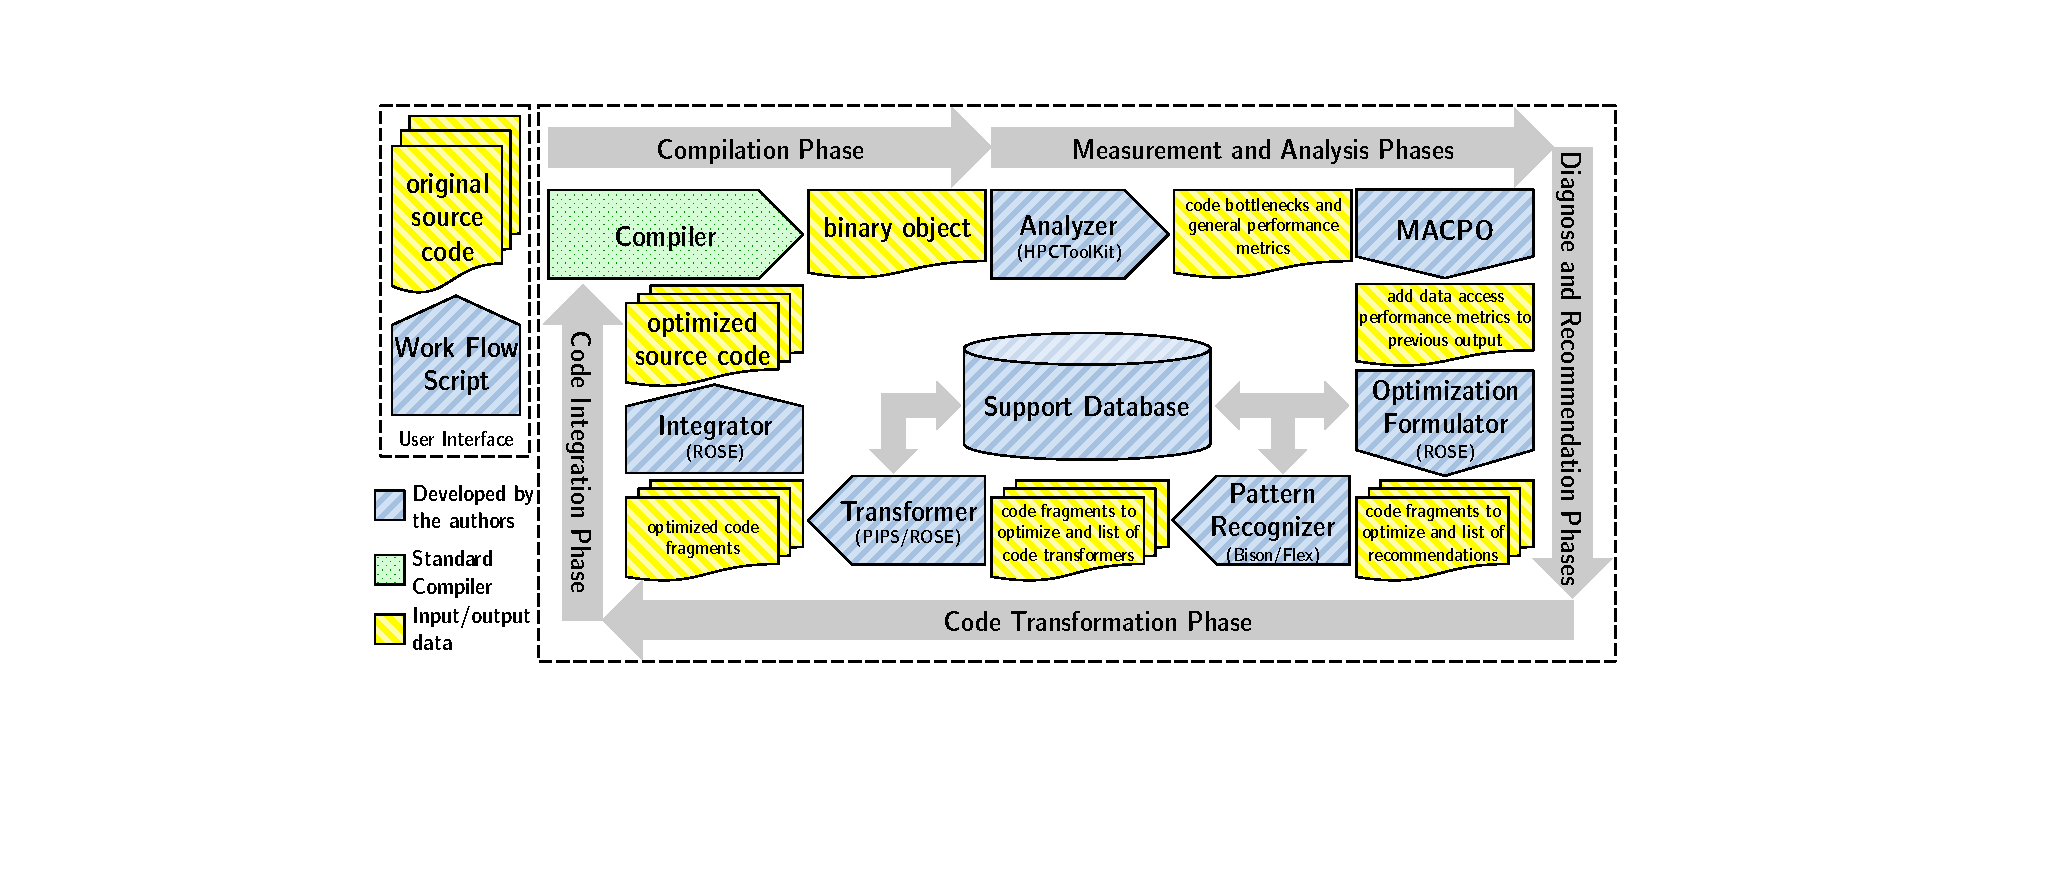
\includegraphics[width=12.8cm]{figures/pe_after}}
	\end{picture} \pause
	\begin{columns}[c]
		\begin{column}{0.86\textwidth}
			\begin{block}{}
				\begin{itemize}
					\item Loads performance metrics on the Support Database \\[2mm] \pause
					\item Runs all \textit{``recommendation selection functions''} \\[2mm] \pause
					\item Concatenates and ranks the list of recommendations \\[2mm] \pause
					\item Extracts code fragments identified as bottlenecks \\[2mm] \pause
					\item Based on ROSE \\[2mm] \pause
					\item \textbf{Extendable:} accepts user-defined performance metrics \\[2mm] \pause
					\item \textbf{Extendable:} it is possible to write new \textit{``recommendation selection functions''} (SQL query) \\[2mm]
				\end{itemize}
			\end{block}
		\end{column}
		\begin{column}{0.19\textwidth}
		\end{column}
	\end{columns}
}

\frame{\frametitle{How PerfExpert does that: Support Database}
	\begin{picture}(0,0)(0,0)
		\put(-28,-160){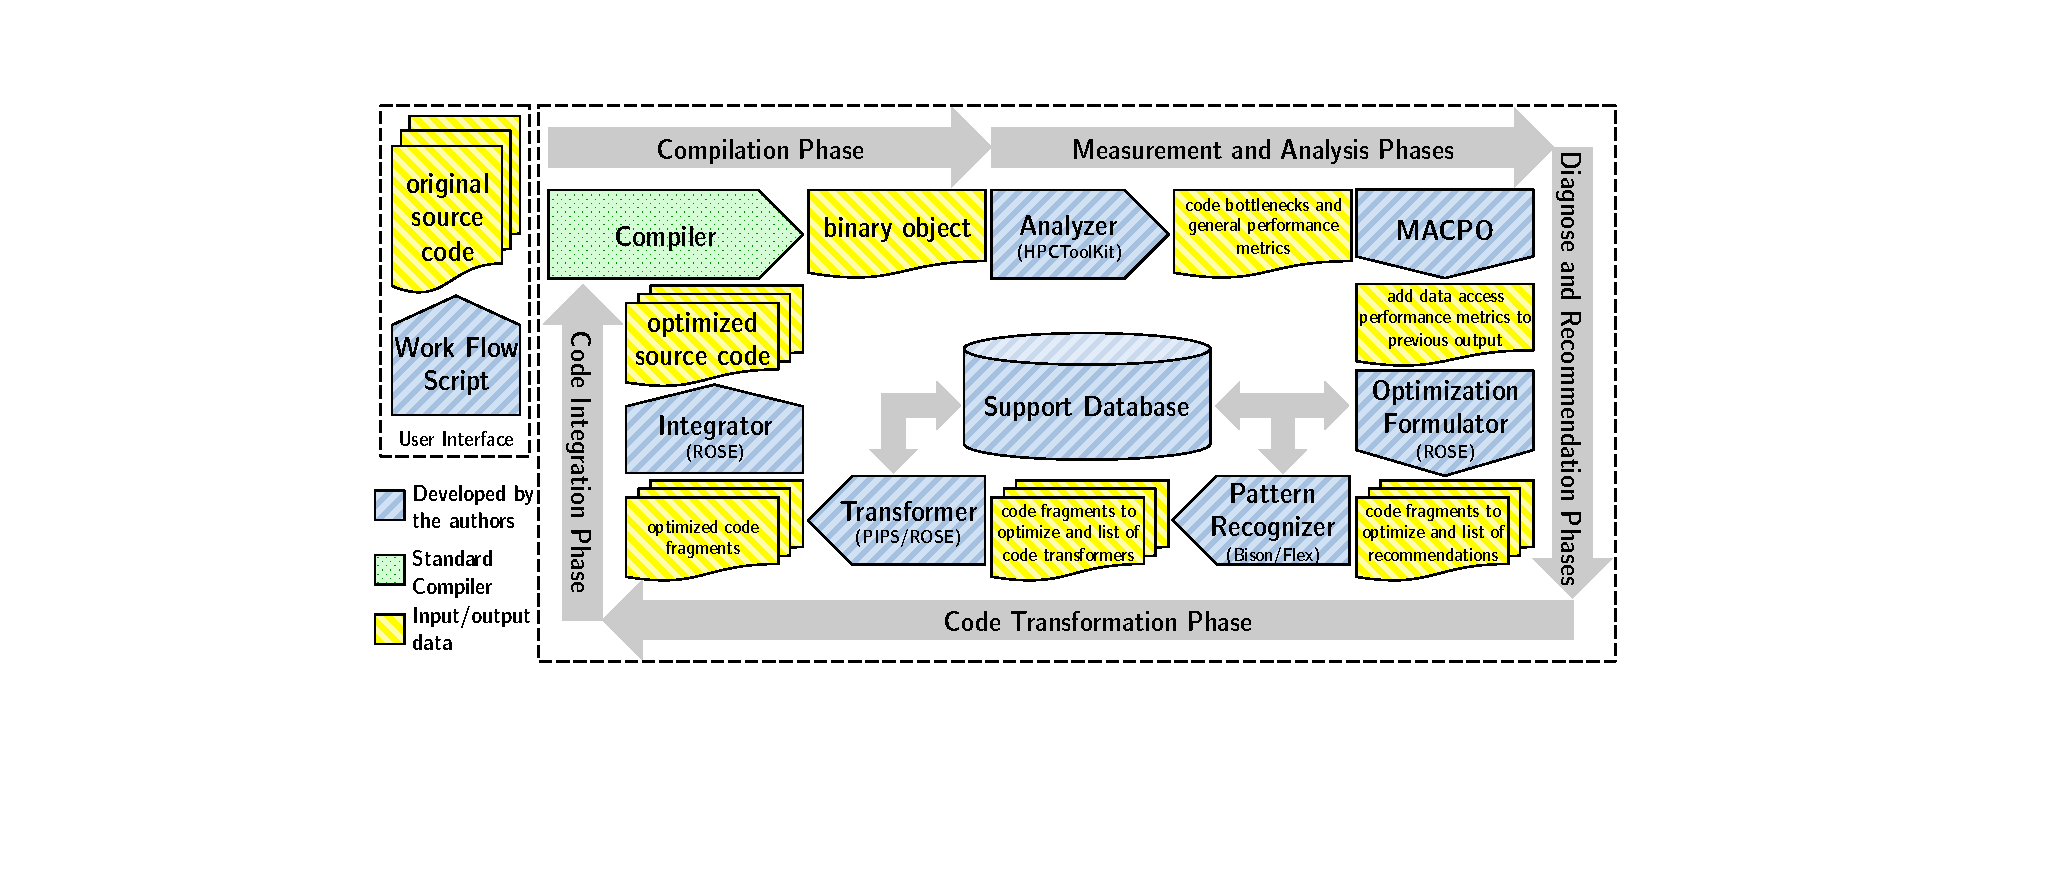
\includegraphics[width=12.8cm]{figures/pe_after}}
	\end{picture} \pause
	\begin{columns}[c]
		\begin{column}{0.1\textwidth}
		\end{column}
		\begin{column}{0.96\textwidth}
			\vspace{-0.8cm}
			\begin{block}{}
				\begin{itemize}
					\item This is a SQLite database \\[2mm] \pause
					\item Stores the list of \textit{``recommendation selection functions''}, \textit{``pattern recognizers''} and \textit{``code transformers''} \\[2mm] \pause
					\item Engine to run the \textit{``recommendation selection functions''}
				\end{itemize}
			\end{block}
		\end{column}
	\end{columns}
}

\frame{\frametitle{How PerfExpert does that: Pattern Recognizer}
	\begin{picture}(0,0)(0,0)
		\put(-28,-160){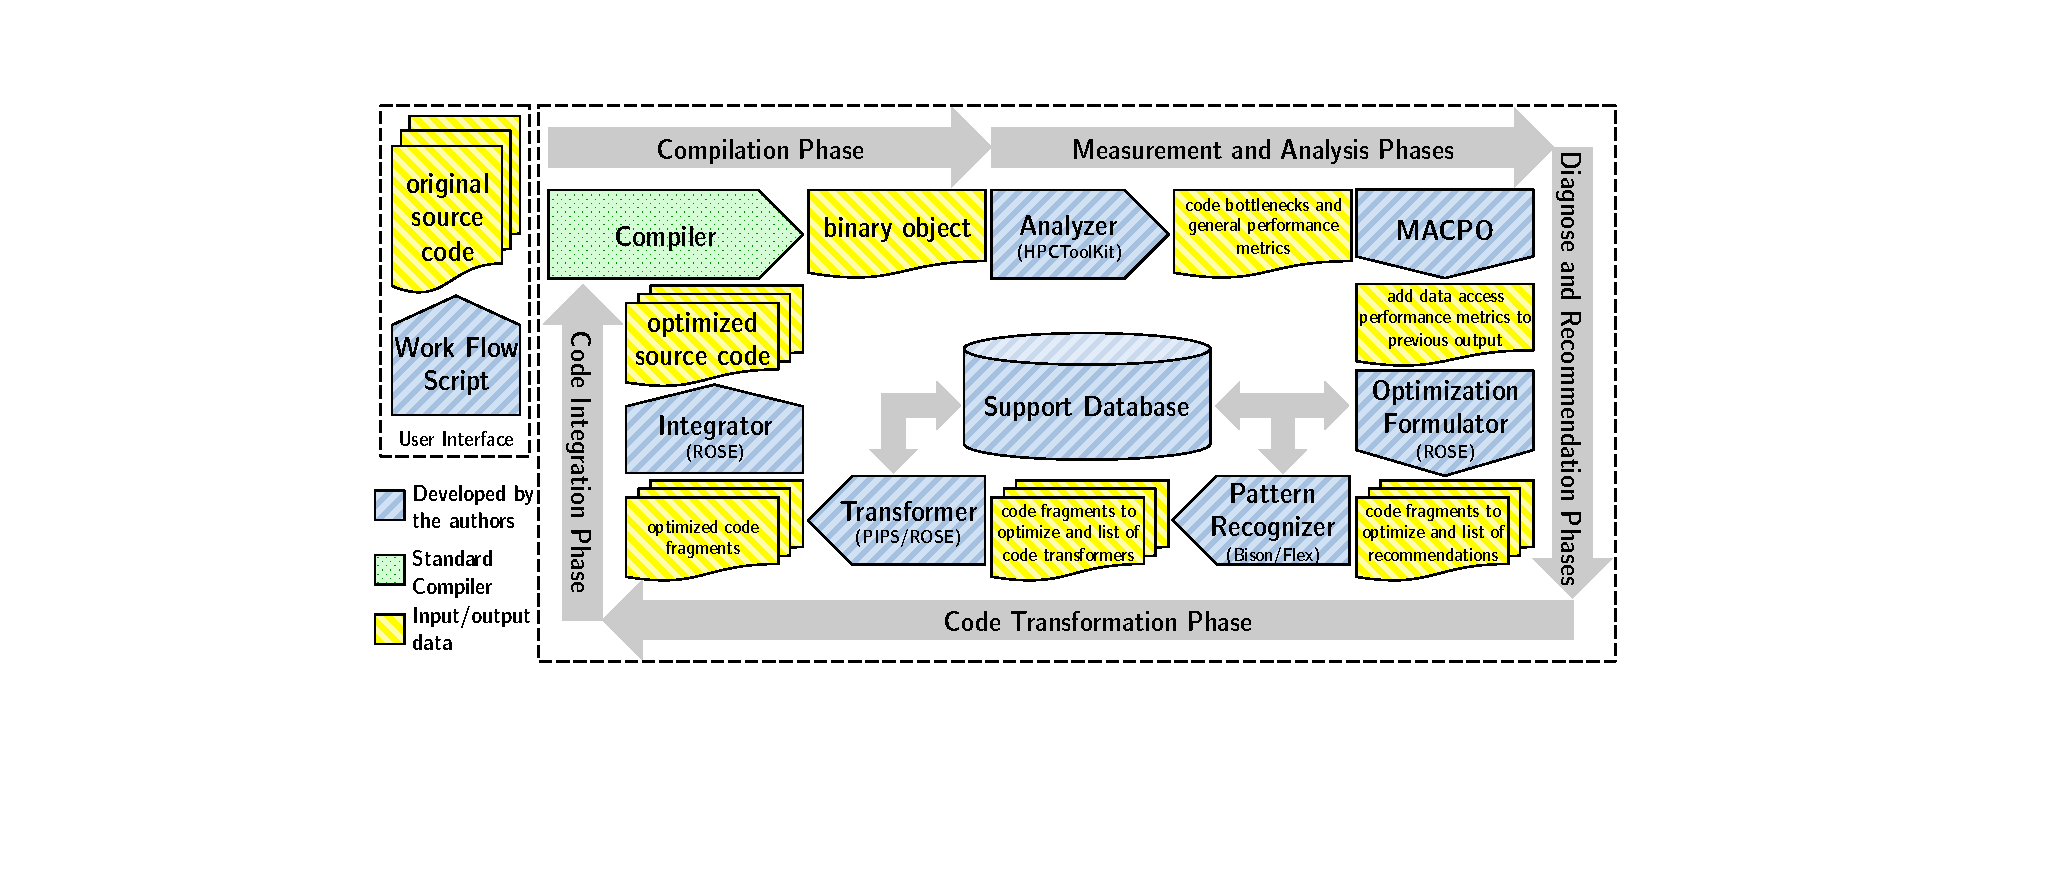
\includegraphics[width=12.8cm]{figures/pe_after}}
	\end{picture} \pause
	\begin{columns}[c]
		\begin{column}{0.05\textwidth}
		\end{column}
		\begin{column}{1.05\textwidth}
			\vspace{-1.2cm}
			\begin{block}{}
				\begin{itemize}
					\item Acts as a ``filter'' trying to find (match) the right code transformer for a source code fragment (identified as bottleneck) \\[2mm] \pause
					\item Language sensitive \\[2mm] \pause
					\item Based on Bison and Flex \\[2mm] \pause
					\item One recommendation may have multiple pattern recognizers \\[2mm] \pause
					\item \textbf{Extendable:} it is possible to write new grammars to recognize/ match/filter code fragments (to work with new ``transformers'') \\[2mm]
				\end{itemize}
			\end{block}
		\end{column}
	\end{columns}
}

\frame{\frametitle{How PerfExpert does that: Transformer}
	\begin{picture}(0,0)(0,0)
		\put(-28,-160){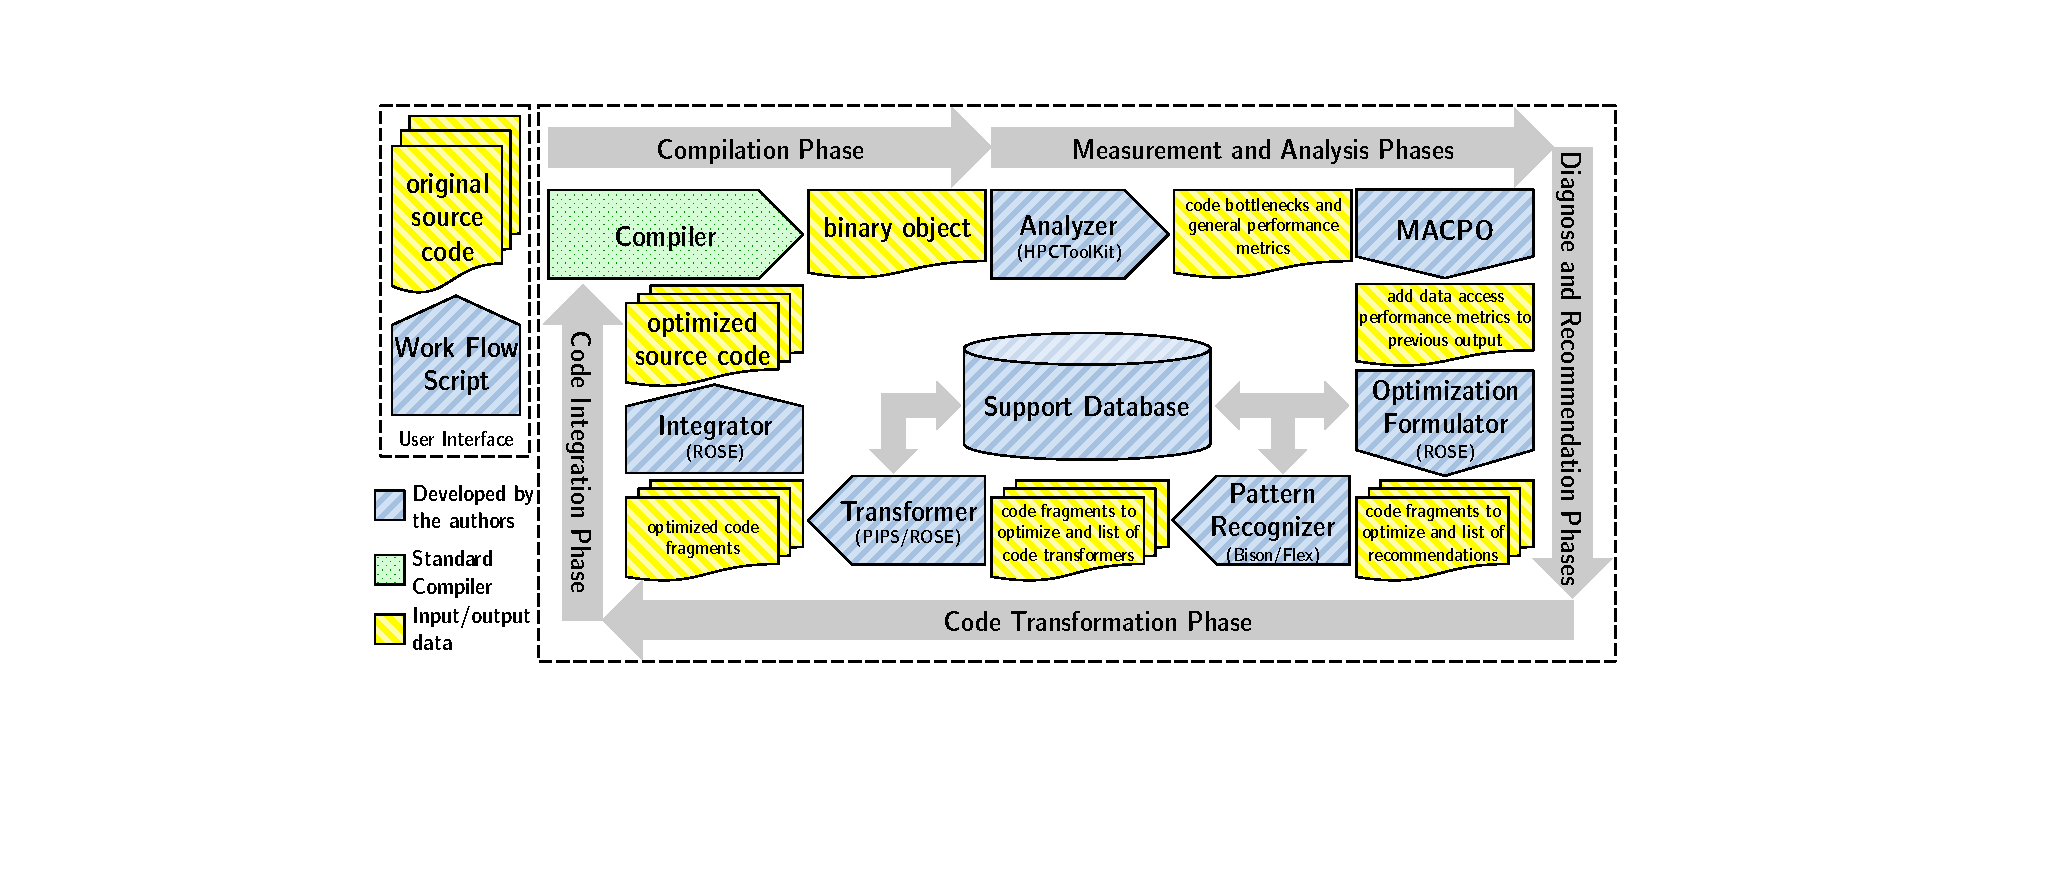
\includegraphics[width=12.8cm]{figures/pe_after}}
	\end{picture} \pause
	\vspace{-1.1cm}
	\begin{block}{}
		\begin{itemize}
			\item Implements the recommendation by applying source code transformation \\[2mm] \pause
			\item May or may not be language sensitive \\[2mm] \pause
			\item Based on ROSE, PIPS or anything you want \\[2mm] \pause
			\item One code pattern may lead to multiple code transformers \\[2mm] \pause
			\item \textbf{Extendable:} it is possible to write code transformers using any language you want \\[2mm]
		\end{itemize}
	\end{block}
}

\frame{\frametitle{How PerfExpert does that: Integrator}
	\begin{picture}(0,0)(0,0)
		\put(-28,-160){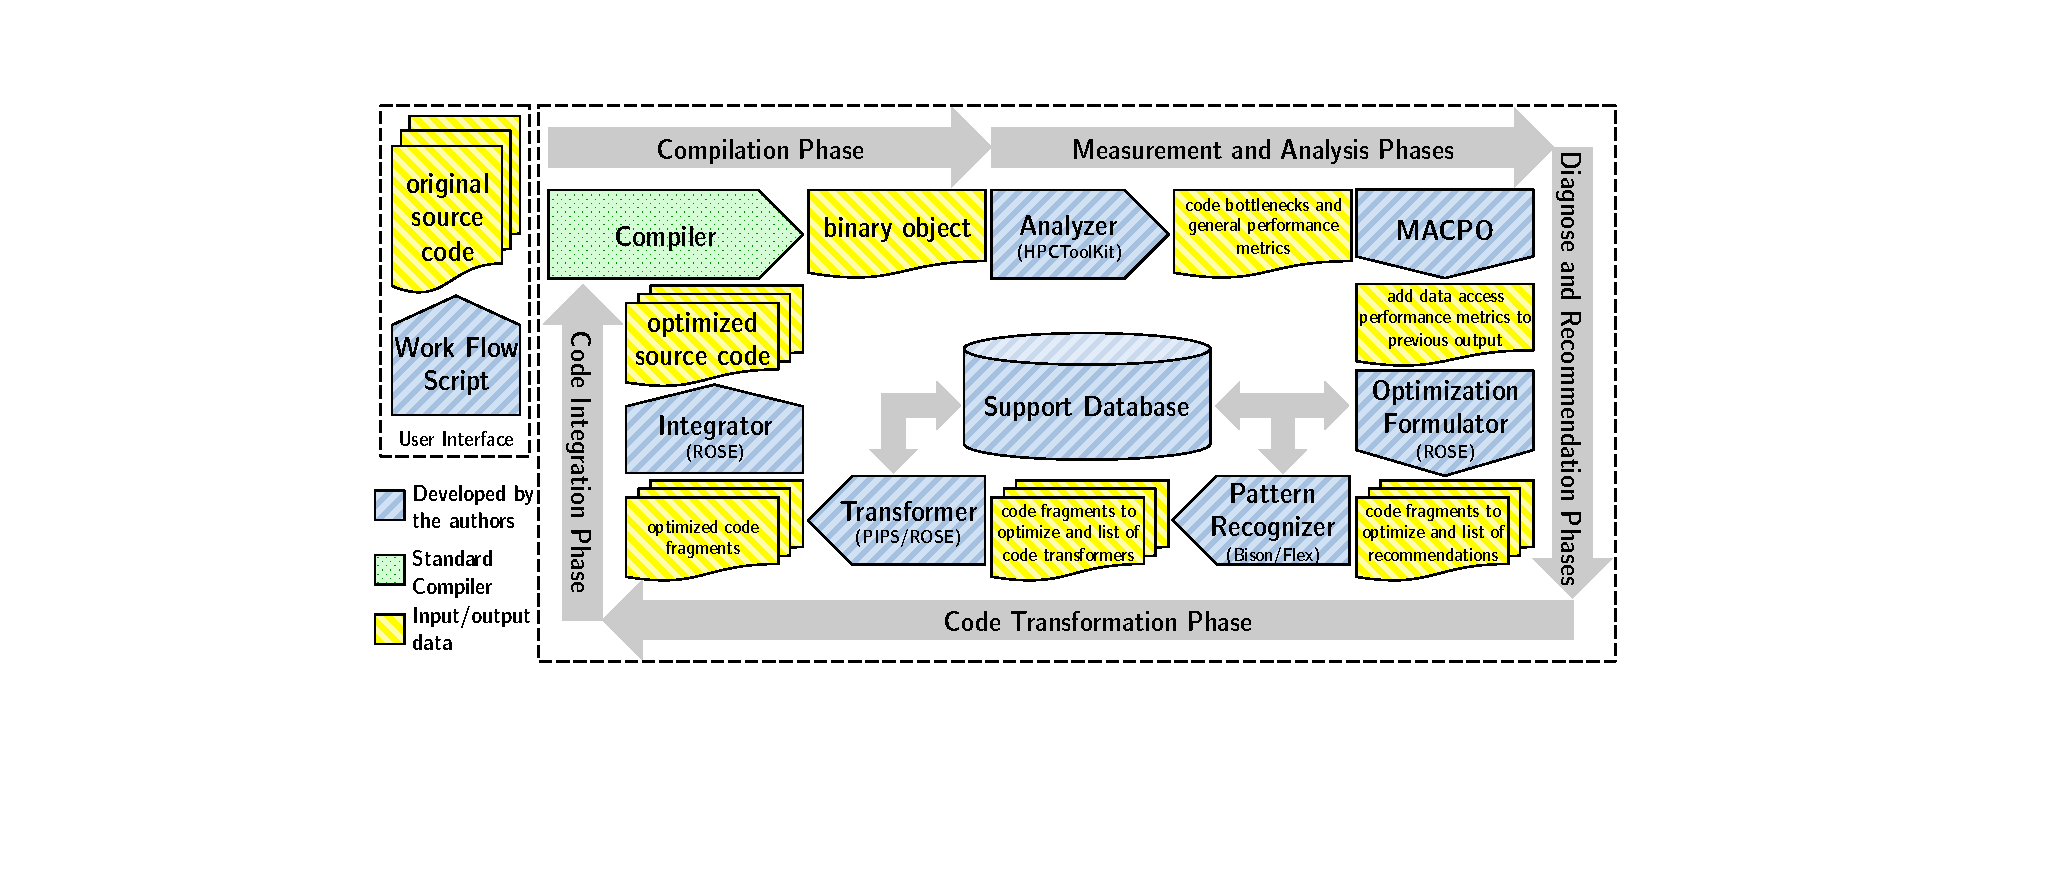
\includegraphics[width=12.8cm]{figures/pe_after}}
	\end{picture} \pause
	\begin{columns}[c]
		\begin{column}{0.35\textwidth}
		\end{column}
		\begin{column}{0.46\textwidth}
			\vspace{1.5cm}
			\begin{block}{}
				\begin{itemize}
					\item Generates a new source code by integrating to the transformed code fragments \\[2mm] \pause
					\item Based on ROSE \\[2mm]
				\end{itemize}
			\end{block}
		\end{column}
		\begin{column}{0.19\textwidth}
		\end{column}
	\end{columns}
}

\frame{\frametitle{How PerfExpert does that: Key Points} \pause
	\begin{block}{Why is this performance optimization ``architecture'' strong?} \pause
		\begin{itemize}
			\item Each piece of the tool chain can be updated/upgraded individually \\[2mm] \pause
			\item It is flexible: you can add new metrics as well as plug new tools to measure application performance \\[2mm] \pause
			\item \textbf{It is extendable}: new recommendations, transformations and strategies to select recommendations (we are counting on you!)\\[2mm] \pause
			\item Multi-language, \textbf{multi-architecture}, open-source and built on top of well-established tools (HPCToolKit, ROSE, PIPS, etc.)\\[2mm] \pause
			\item Easy to use and lightweight!
		\end{itemize}
	\end{block}
}

\subsection{Extending PerfExpert}

\frame{\frametitle{Extending PerfExpert} \pause
	\begin{block}{} \pause
		\begin{itemize}
			\item Adding performance metrics \\[2mm] \pause
			\item Optimization recommendations [entries on the SQL database]\\[2mm] \pause
			\item ``Recommendation selection functions'' \\[2mm] \pause
			\item Pattern recognizers \\[2mm] \pause
			\item Code transformers \\[2mm]
		\end{itemize}
	\end{block}
}

\frame{\frametitle{Extending PerfExpert} \pause
	\begin{block}{Adding Performance Metrics} \pause
		\texttt{\small code.section\_info=Loop in function compute() at mm.c:8\\
code.filename=mm.c\\
code.line\_number=8\\
code.type=loop\\
code.function\_name=compute\\
code.extra\_info=3\\
code.representativeness=99.8\\
perfexpert.ratio.data\_accesses=0.25\\
perfexpert.instruction\_accesses.L2i\_hits=0.002\\
perfexpert.branch\_instructions.mispredicted=0.0\\
perfexpert.floating-point\_instr.fast\_FP\_instr=5.073\\
perfexpert.data\_accesses.L2d\_hits=1.846\\...\\}
	\end{block}
}

\frame{\frametitle{Extending PerfExpert} \pause
	\begin{block}{Recommendation Selection Functions} \pause
		\texttt{\small SELECT r.id AS recommendation\_id, SUM(\\
\ \ (CASE c.short WHEN 'd-l1' THEN\\
\ \ \ \ (m.data\_accesses\_L1d\_hits - (max * 0.1))\\
\ \ \ \ ELSE 0 END) +\\
\ \ \ \ ... ) AS score FROM recommendation AS r\\
JOIN metric AS m JOIN (SELECT MAX(\\
\ \ m.data\_accesses\_L1d\_hits, m.data\_accesses\_L2d\_hits,\\
\ \ ... ) AS max\\
\ \ FROM metric AS m WHERE m.overall * 100 /\\
\ \ \ \ (0.5 * (100 - m.ratio\_floating\_point) +\\
\ \ \ \ m.ratio\_floating\_point) > 1\\
\ \ AND m.id = @RID)\\
WHERE (r.loop <= @LPD AND m.code\_type = 'loop') OR\\
\ \ (r.loop IS NULL AND m.code\_type = 'function')\\
\ \ AND m.id = @RID\\
GROUP BY r.id ORDER BY score DESC;
}
	\end{block}
}

\frame{\frametitle{Extending PerfExpert} \pause
	\begin{block}{Pattern Recognizers} \pause
		\texttt{\tiny nested\_iteration\_statement\\
 : WHILE '(' exp ')' WHILE '(' exp ')' stmnt\\
 | WHILE '(' exp ')' '{' WHILE '(' exp ')' stmnt '}'\\
 | DO DO stmnt WHILE '(' exp ')' ';' stmnt WHILE '(' exp ')' ';'\\
 | DO '{' DO stmnt WHILE '(' exp ')' ';' '}' WHILE '(' exp ')' ';'\\
 | FOR '(' exp\_stmnt exp\_stmnt ')' FOR '(' exp\_stmnt exp\_stmnt ')' stmnt\\
 | FOR '(' exp\_stmnt exp\_stmnt ')' '{' FOR '(' exp\_stmnt exp\_stmnt ')' stmnt '}'\\
 | FOR '(' exp\_stmnt exp\_stmnt exp ')' FOR '(' exp\_stmnt exp\_stmnt exp ')' stmnt\\
 | FOR '(' exp\_stmnt exp\_stmnt exp ')' '{' FOR '(' exp\_stmnt exp\_stmnt exp ')' stmnt '}' ;\\
}
	\end{block}
}

\frame{\frametitle{Extending PerfExpert} \pause
	\begin{block}{Code Transformers} \pause
		\texttt{\small create c\_loop2 ../source/mm.c\\
activate INTERPROCEDURAL\_SUMMARY\_PRECONDITION\\
activate TRANSFORMERS\_INTER\_FULL\\
activate PRECONDITIONS\_INTER\_FULL\\
setproperty SEMANTICS\_FIX\_POINT\_OPERATOR ``derivative''\\
module compute\\
apply LOOP\_INTERCHANGE\\
loop\_8\\
apply UNSPLIT[\%PROGRAM]\\
close\\
quit\\
}
	\end{block}
}

\subsection{Hands on Tutorial: PerfExpert}

\frame{\frametitle{Hands on Tutorial}
	\begin{block}{Accessing Stampede:}
		\begin{itemize}
			\item \texttt{ssh login@stampede.tacc.utexas.edu} \\[2mm]
			\item use the password that has been provided to you
		\end{itemize}
	\end{block}

	\begin{block}{Request a Compute Node:}
		\begin{itemize}
			\item \texttt{./reserve} \\[2mm]
			\item now we are ready to go...
		\end{itemize}
	\end{block}
}

\frame{\frametitle{Hands on Tutorial}
	\begin{block}{Accessing Stampede:}
		\begin{itemize}
			\item \texttt{cd 1} \\[2mm]
			\item \texttt{perfexpert} \\[2mm]
			\item \texttt{perfexpert -s mm.c mm} \\[2mm]
			\item \texttt{grep -R "running time" *} \\[2mm]
			\item \texttt{more mm.c} \\[2mm]
			\item \texttt{more perfexpert-temp-zUKfkx7/1/fragments/new/mm.c} \\[2mm]
			\item \texttt{perfexpert mm} \\[2mm]
			\item \texttt{perfexpert -r 5 mm} \\[2mm]
			\item \texttt{cd ../2} \\[2mm]
			\item \texttt{perfexpert -m -s backprop.c backprop}
		\end{itemize}
	\end{block}
}

\subsection{Morning Closure}

\frame{\frametitle{Agenda} \pause
	\begin{block}{What we saw in the morning:}
		\begin{itemize}
			\item Introduction and motivation \\[2mm] 
			\item What PerfExpert can provide to you? \\[2mm]
			\item Demo \\[2mm]
			\item How PerfExpert does that? (opening Pandora's box) \\[2mm]
			\item Extending PerfExpert \\[2mm]
			\item Hands on tutorial \\[2mm]
			\item Morning closure \\[2mm]
		\end{itemize}
	\end{block} \pause

	\begin{alertblock}{What we will see in the afternoon:}
		How to enhance the application performance using memory access metrics (MAPCO)
	\end{alertblock}
}

%------------------------------------------------------------
\section{MACPO}
\subsection{What PerfExpert can provide to you?}

\subsection{Demo: MACPO}

\frame{\frametitle{Short Demo}
	\vspace{2.5cm}
	\begin{center}
		\textit{\textbf{\Huge{Short demo}}}
	\end{center}
}

\subsection{How MACPO does that?}

\subsection{Hands on Tutorial: MACPO}

\subsection{Enhancing PerfExpert with MACPO analysis}

\section{GPU/Accelerators}
\subsection{GPU/Accelerators}

\frame{\frametitle{Performance Optimization by Mapping to Accelerators} \pause
	\begin{block}{} \pause
		{\Large Mapping of code segments to accelerators is  becoming one of the most methods for optimizing the performance of an application}
	\end{block}

	\begin{alertblock}{} \pause
		{\Large \textbf{Problem:} how to select those parts of an application which will benefit from execution on an accelerator?}
	\end{alertblock}
}

\frame{\frametitle{Code Segments for SIMT/SIMD Execution} \pause
	\begin{block}{}\small \pause
		\begin{itemize}
			\item Optimize for multicore chip execution --- \textbf{PerfExpert, why?} \\[2mm] \pause
			\item Identify time consuming kernels in code --- \textbf{PerfExpert} \\[2mm] \pause
			\item Eliminate kernels not easily mappable for SIMT/SIMD execution --- \textbf{How?} \\[2mm] \pause
			\item Characterize the kernels suitable for SIMT/SIMD execution --� \textbf{What properties?} \\[2mm] \pause
			\item Rank appropriate kernels using the characteristics identified in the last step \\[2mm] \pause
			\item Estimate cost of data movement \\[2mm] \pause
			\item Look for refactorings that will enable leaving data on accelerator \\[2mm] \pause
			\item Generate compiler annotations for translation of C/C++/Fortran to CUDA/OpenCL \\[2mm] \pause
			\item Suggest kernels needing new algorithms \\[2mm]
		\end{itemize}
	\end{block}
}

\frame{\frametitle{Code Segments for SIMT/SIMD Execution} \pause
	\begin{block}{Unsuitable Kernels} \pause
		\begin{itemize}
			\item Frequent TLB misses \\[1mm] \pause
			\item High fraction of branches \\[1mm] \pause
			\item Cache conflicts across cores \\[1mm] \pause
			\item Irregular access strides for kernel data structures \\[1mm]
		\end{itemize}
	\end{block}

	\begin{block}{Characterizing ``Good'' Kernels} \pause
		\begin{itemize}
			\item Computational intensity \\[1mm] \pause
			\item Pure ``local'' SPMD parallelism \\[1mm] \pause
			\item Streaming parallelism or vectorization \\[1mm] \pause
			\item Regular access strides for data structures \\[1mm] \pause
			\item Data reuse factor and data transfer volume \\[1mm] \pause
			\item ``Limited'' recursion \\[1mm]
		\end{itemize}
	\end{block}
}

\frame{\frametitle{Code Segments for SIMT/SIMD Execution} \pause
	\begin{block}{Ranking ``Good'' Kernels} \pause
		\begin{itemize}
			\item Curve fit characteristics to speed-up measurements of kernels that have already been mapped \\[2mm] \pause
			\item Sort by values of characteristics in some chosen order \\[2mm] \pause
			\item Hold up your thumb? \\[2mm]
		\end{itemize}
	\end{block}
}

\frame{\frametitle{Example} \pause
}

\subsection{Selecting code segments to run on GPUs/accelerators}

\section{Closure}

\subsection{Afternoon Closure}

%------------------------------------------------------------
%\section{Conclusions}
%\subsection{Conclusions}
%\frame{\frametitle{Conclusions} \pause
%	\begin{block}{}
%		\begin{itemize}
%			\item This is the first end-to-end open-source performance optimization tool (as far as we know)\\[2mm] \pause
%			\item It will become more and more powerful as new recommendations, transformations and features are added \\[2mm] \pause
%			\item Different from (most of) the available performance optimization tools, there is no ``big code'' (to increase in complexity until it become unusable or too hard to maintain) \\[2mm]
%		\end{itemize}
%	\end{block}
%}
%
%\frame{\frametitle{Next Steps} \pause
%	\vspace{-0.4cm}
%	\begin{block}{Major Goals}\small \pause
%		\begin{itemize}
%			\item Improve analysis based on the data access (short term) \\[1mm] \pause
%			\item Increase the number of recommendations and possible code transformations (continuously) \\[1mm] \pause
%			\item New algorithms for recommendations selection (short term) \\[1mm] \pause
%			\item Add support to MPI-related recommendations (medium term) \\[1mm] \pause
%			\item Add support to MPI-related code transformations (long term) \\[1mm] \pause
%		\end{itemize}
%	\end{block}

%	\begin{block}{Minor Goals}\small \pause
%		\begin{itemize}
%			\item Support ``Makefile''-based source code/compilation tree \\[1mm] \pause
%			\item Make the required packages installation process easier \\[1mm] \pause
%			\item Add a test suite based on established benchmark codes \\[1mm] \pause
%			\item Easy-to-use interface to manipulate the support database \\[1mm]
%		\end{itemize}
%	\end{block}
%}

\frame[plain]{
	\vspace{3cm}
	\begin{center}
		\textbf{\Huge{Thank You}}
	\end{center}
	\vspace{2cm}
	\pgfuseimage{logo_TACC} \ \ \pgfuseimage{logo_UT}
}

%------------------------------------------------------------
\end{document}